% ========== SORTKRAGE ==========
\begin{frame}{%
  \begin{minipage}[c]{0.30\textwidth}
    Sortkrage (Krage)
  \end{minipage}%
  \hfill
  \begin{minipage}[c]{0.45\textwidth}
    \footnotesize
    \textbf{Jagttid:} 1.\ september -- 31.\ januar
  \end{minipage}%
  \hfill
  \begin{minipage}[c]{0.15\textwidth}
    \noindent\raggedleft
    
\includegraphics[width=0.5cm, height=0.5cm, keepaspectratio]{Billeder/Ikoner/star.png}%
    \hspace{0.2em}%
    
\includegraphics[width=0.5cm, height=0.5cm, keepaspectratio]{Billeder/Ikoner/star.png}%
    \hspace{0.2em}%
    
\includegraphics[width=0.5cm, height=0.5cm, keepaspectratio]{Billeder/Ikoner/star.png}
  \end{minipage}%
}
  \vspace{0.25em}
  \begin{columns}[T]
    \column{0.45\textwidth}
    \setlength{\parskip}{0.45em}
    \tiny
    \RaggedRight
    \textbf{\textit{Corvus corone}} – mellemstor kragefugl, nært beslægtet med gråkrage \par
    \textbf{Udseende:}\\
    \quad – Heltsort krop og hoved \\
    \quad – Sorte øjne \\
    \quad – Ligner ravn, men er mindre og har slankere næb \par
    \textbf{Levesteder:} Alle landskabstyper. \par
    \textbf{Føde:} Opportunist – spiser alt, inkl.\ yngel. \par
    \textbf{Udbredelse:} Især Vestjylland. Sjældnere i resten af landet. \par
    \textbf{Træk/standfugl:} Begge \par
    \textbf{Forplantning:}\\
    \quad – \textbf{Yngleforhold:} Yngler i høje træer. Parret forsvarer territoriet \\
    \quad – \textbf{Kønsmoden:} 2 år \\
    \quad – \textbf{Mono/polygam:} Monogam \\
    \quad – \textbf{Bestandsomsætning:} Langsom \\
    \quad – \textbf{Kuld:} 4--6 æg
    \column{0.52\textwidth}
    \centering
    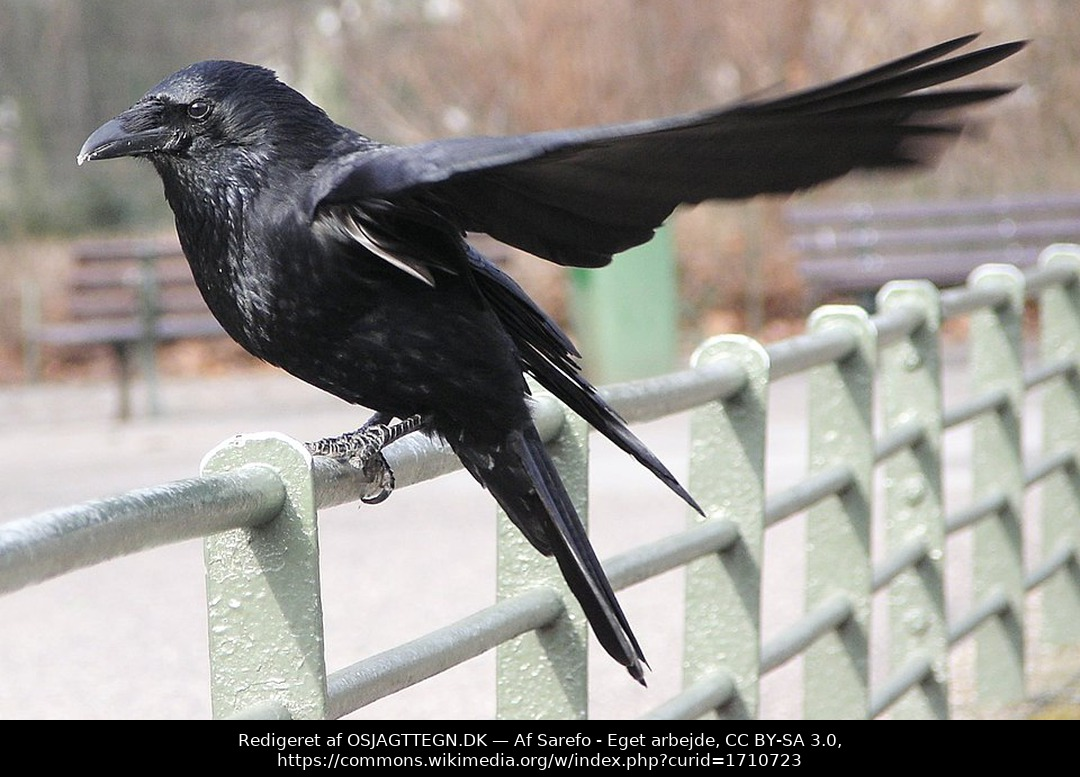
\includegraphics[width=\linewidth, height=7.2cm, keepaspectratio]{Billeder/Dyr/Fugle/Spurvefugle/sortkrage-01.jpg}
  \end{columns}
\end{frame}